\chapter{KWS and SV Models}
\label{cha:training} 
\section{KWS Model}
\label{sec:kws deployment}
• Edge Impulse Integration - Model training and validation\newline
• C implementation, direct MFE computation on device\newline
• KWS model Deploying (Edge Impulse)\newline
Input (1600) → FC256 (ReLU) → FC256 (ReLU) → FC256 (ReLU) → Output (4, Softmax)\newline
Simulation (Weight extraction, target word, dataset), Real (model uploading and classification method)\newline

\newpage
PAGE 2
\newpage
PAGE 3
\newpage
\section{SV Model}
\label{sec:sv introduction}
After creating the KWS model, the objective is creating a text-dependent Speaker Verification model, which requires only one train. This is known as ASV (Adaptive Speaker Verification), which relies on comparing the results of the model (d-vectors) with reference samples stored in system dataset, which have to be captured during inference phase. Speaker Verification is used in recognizing the identity of a user in a on-device learning context. To approach this way a large amount of data is required at first to train the model, performing a meticulous extraction of d-vectors to recognize patterns in user voice and possibly trying to minimize the required number of samples, maximizing the security recognition. A sample, because of text-depencendy, will correspond to a word said by one user and should compare only with its similar.\newline
The deployment of the model requires 3 caveats:\newline
1. Adapting directly on device, meaning that a new user should be able to enroll in SV application by providing samples of its voice in real time through the target device\newline
2. The algorithm has to operate in one-class manner and it should be able to learn to distinguish between the enrolled user and the others, only using the data from the dataset collected during inference\newline
3. To be fit in a TinyML device the considerations should be done in memory allocation depending on the device used, so the model should fit in Flash Memory\newline
To obtain the desired d-vector we should use a convolutional neural network, because we would like to reduce dimensionality, while obtaining significantly features. This is achieved with some expensive filters that while reducing width and heights, will generating new channels corresponding to a new feature extracted. This is a way to synthesize the input spectrogram (40 width x 40 height x 1 channel) to a lower dimension.\newline
A valid alternative, in theory, could be i-vectors. It is a feature that represents the characteristics of frame-level features distributive pattern. The extraction is a dimensionality reduction of GMM supervector, allowing an extraction per sentence, instead d-vector generates one-hot speaker label on the output and it is an averaged activation from the last hidden layer of CNN. The advantage of d-vector is that there is no assumption on feature's distribution, instead i-vector assumes as default a Gaussian distribution.
\subsection{Model Creation}
\label{subsec:model creation}
The structure of the CNN follows the theoretical one introduced and as input is given the spectrogram given in output from MFE block (40x40x1) and as output the objective is a 256-size long array of relevant features (d-vector). However, it cannot be the model output, because at first the model should classify the data given in input, through a fully connected layer. As input dataset is used a huge one with many different speakers and each providing various samples, because they comes from audio book recording. From speakers classification is not required the text-dependent approach, so the speakers will say many different words, which helps in generate the required weights and biases for the convolution layers. The dataset used was from libreSpeech which has data collected per speaker and for the purpose was taken the one with 100 hours clean speech in English Language sampled with 16kHz, which is the same of Syntiant audio processing\cite{librispeech}, corresponding to ~6GB memory space to make the training successful in reasonable times.\newline
A first problem is that these samples are not already in 1 second, but variable, so they have been sampled and the parsed through the MFE Block previously introduced. The total spectrograms obtained were 136112 for a total number of classes of 94 and a total of ~38 hours of recording and a memory occupation of 871MB. To have a balanced dataset all classes had the number same samples 1448 as fact at first should have been 100, but they had too few samples. A convolution Neural should perform 3 actions during its creation in which the dataset should subdivide its samples:\newline
1. Training - The spectrogram is threated as an image, this dataset is the base of the model and on these the weights are adjusted using backpropagation, like Adam optimizer, and using loss functions like cross-entropy, for classification, or MSE, for regression, to minimize the failure rate. It uses a learning rate, which is a hyperparameter, determining the step size at each iteration while moving forward with epochs. A epoch consists in a cycle of training input processing and an evaluation and can be arbitrary set according to the complexity of the network. In this case, it was set to 700.
2. Validation - This is used to see the result on data other than the ones in training set. It is used to adjust learning rate and batch size in case it starts overfitting or perform an early stopping if validation loss increases.
3. Testing - It is a dataset to which are added background noise, varying microphone quality and other modifications to the original input. It is like a validation, but is to stress-out the system and seeing if it can still working with some fluctuations.\newline
The distribution among these 3 sets is random inside a class, but each one will have an amount in each set. For precision, 70\% of samples will go in training (95278), 15\% in validation (20417) and 15\% in testing (20417). In training with CNN is suggested to avoid fluctuations a batch size and considering that the samples may not be complete words it performs an attenuate on those cases and the objective in having a good identification of the speaker. Knowing that a higher batch size will provide more accuracy, it was chosen 32 size, which should be stable with standard learning functions.\newline
The setup of the model, as summary, is an input shape of (32,40,40,1) [batch,width,height,channel] for 2977 inputs (95278/32) and output shape of 94 classes. The model creation required about 3 hours using a GPU. The proposed architecture is the following\cite{dvector_extractor_TinySV}:
\begin{center}
    \begin{figure}[!h]
        \centering
        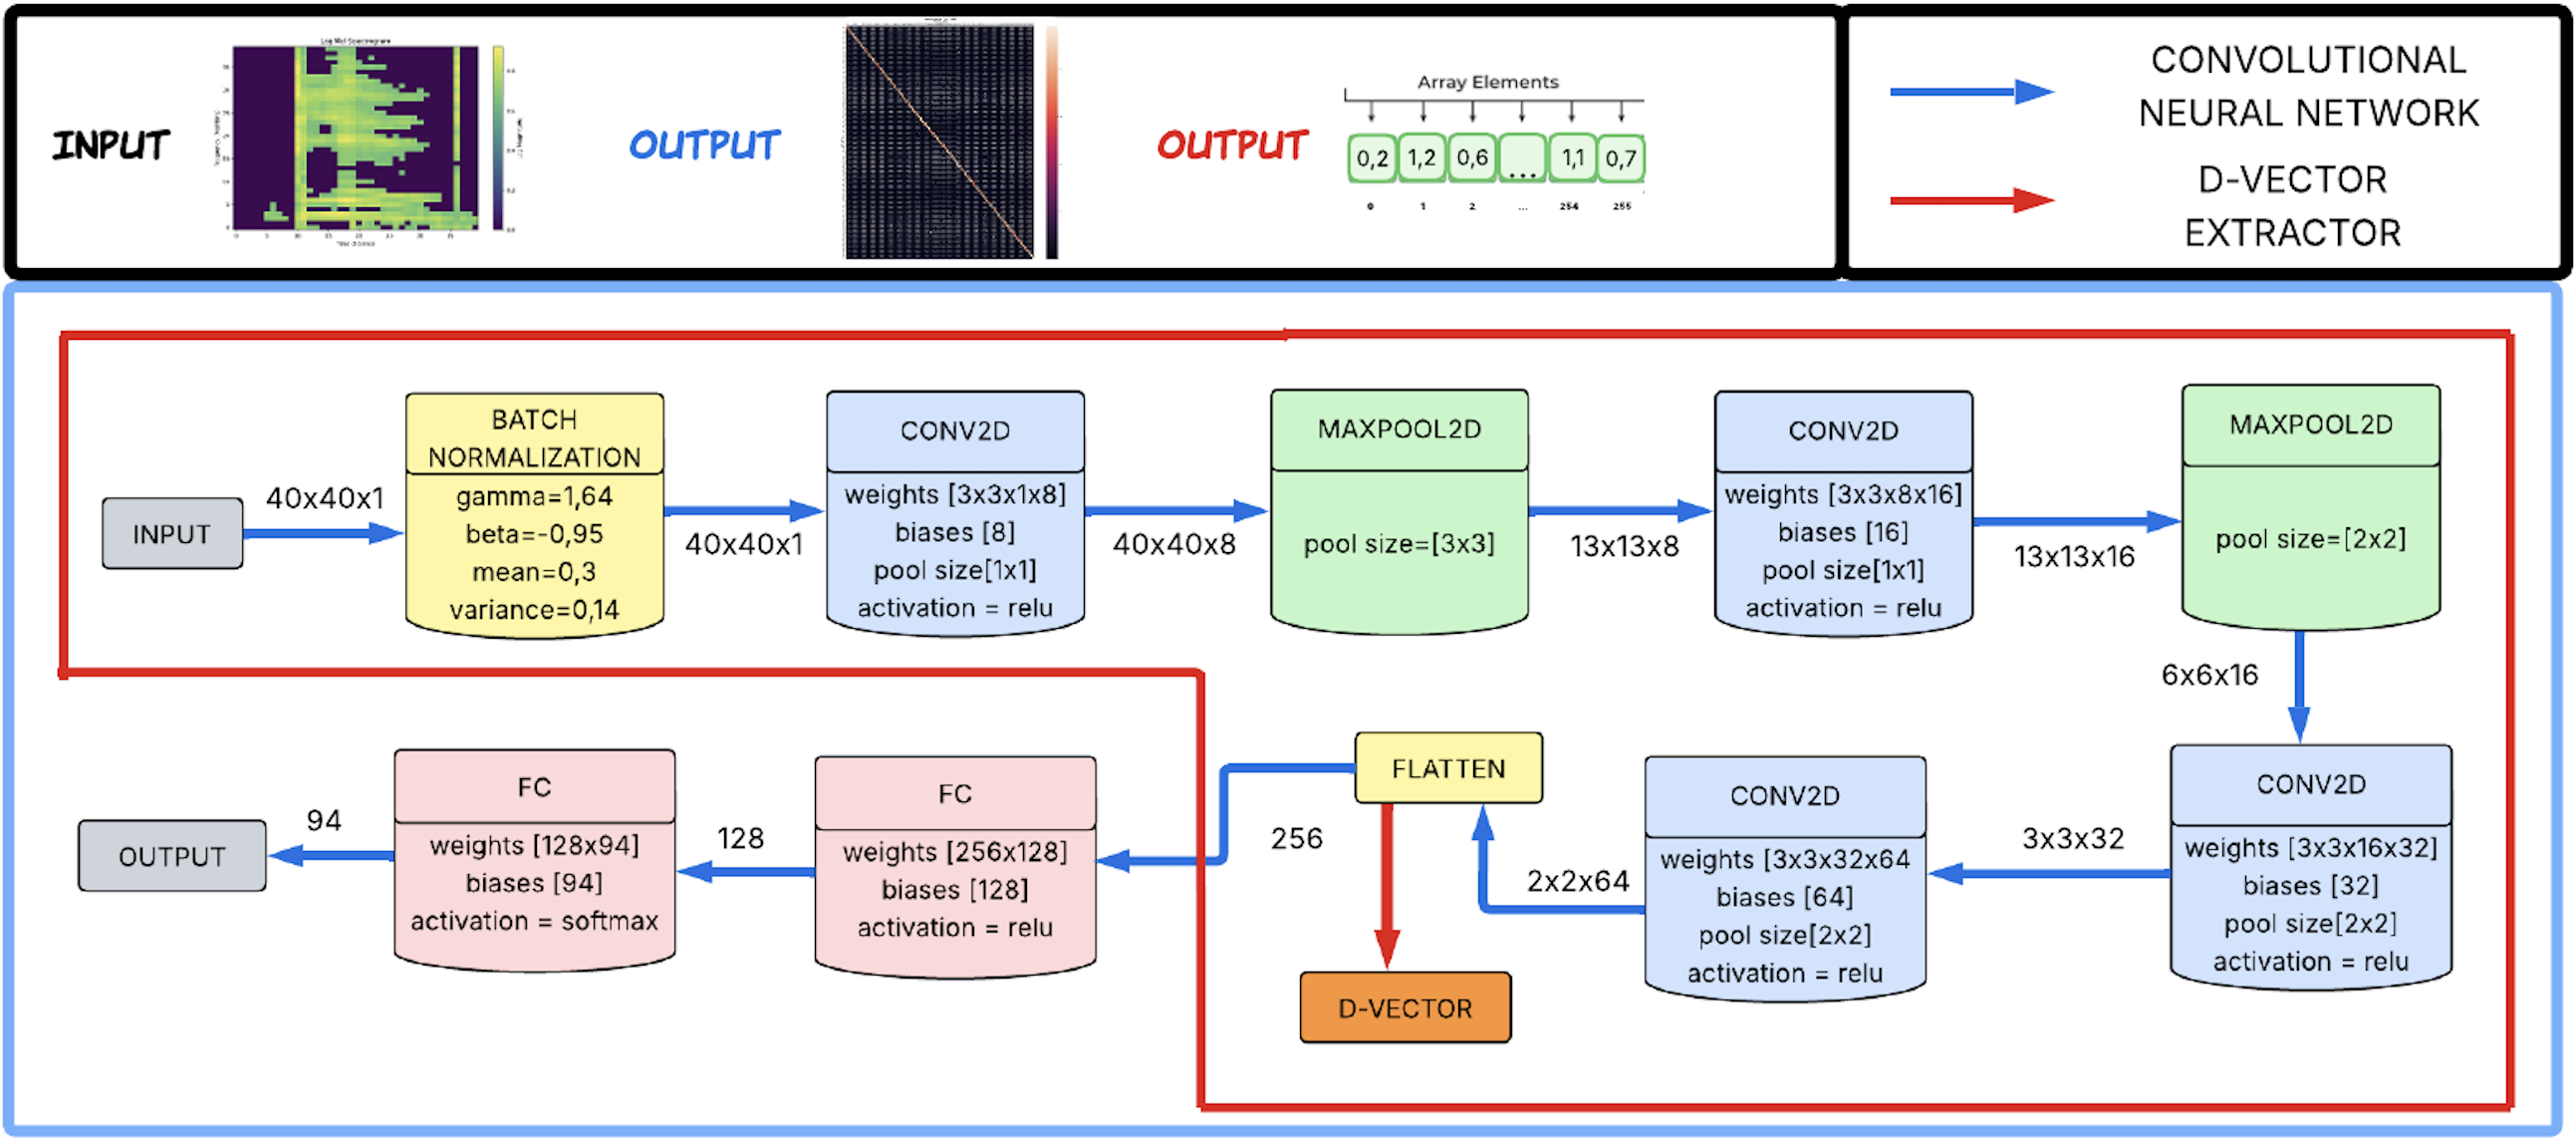
\includegraphics[width=1.0\textwidth]{images/3.01 D-vector Extractor.png}
        \caption{Speaker Verification Neural Network and D-vector Extractor}
    \end{figure}
\end{center}

\subsection{Knowledge Distillation Training}
• Database design for sample saving \newline
• Cosine similarity EER \newline
• Extend functionality to SV to be compatible with device (Python)\newline
Input (40x40) → Conv+BatchNorm layers → 256-dimensional d-vector \newline
Simulation (model-size, classification purpose, truncation explaination, verification methods (best-matching and mean-cosine)), Real (custom logic for verification)\newline

\subsection{Quantization of SV Model}
\label{sec:quantization}
• Float32 → Int8: Performance metrics showing minimal accuracy loss\newline
• Int8 → Int4: Challenges in maintaining model quality\newline
• Performance Comparison:\newline
    - Original CNN model vs. distilled DNN\newline
    - Full-precision vs. quantized implementations\newline
• Optimize neural network to be deployed on the device and verifying on simulation (Syntiant NDP101 and C-code)\newline\newline

\newpage
PAGE 6
\newpage 
PAGE 7
\newpage 